\documentclass[aps,prb,onecolumn,superscriptaddress]{revtex4-2}
\usepackage{amsmath,amssymb,graphicx,booktabs}
\begin{document}
\title{Occupied-Frame Validation for a U(1)-Symmetric Gaussian Transfer Circuit}
\author{Automated validation campaign}
\date{\today}
\begin{abstract}
We validate a frame-native implementation of the canonical CPU Markov circuit against its rank-one covariance implementation at $N_x=N_y=16$ for random pure and maximally mixed initial states. The first physics gate is a uniform $\alpha=1$, domain-wall-free Chern insulator. The combined numerical and physics gate passed. Performance data, when present, are descriptive and are not part of implementation validity.
\end{abstract}
\maketitle

\section{Representation and update rules}
For a pure physical Gaussian state, the occupied frame $V\in\mathbb C^{N\times r}$ obeys $V^\dagger V=I$ and $C=VV^\dagger$. For a mixed physical state we use a doubled pure frame $F=(A;B)$ with $C=BB^\dagger$; maximal mixing starts from $F=2^{-1/2}(I;I)$. Given a normalized orbital $e$, gain uses $z=F^\dagger e$, $h=e-Fz$, and appends $h/\lVert h\rVert$. Loss builds a stable complex Householder reflector taking $z$ to the last coefficient coordinate, applies its rank-one right action, and deletes the final column. Correct occupied and empty projections are chronological loss--gain and gain--loss words. Under perfect correction, mismatches reduce to a bare loss or gain.

The evolution kernel evaluates overlaps from the local $n_{\rm shell}=1$ support. It performs no covariance construction, pseudoinverse, or global QR. Covariance and doubled-projector construction occur only in the instrumented correctness observers and declared checkpoints; those costs are excluded from update-only benchmark timing.

\section{Campaign design}
The locked campaign uses $N=512$ physical orbitals, 32 cycles, complex128 arithmetic, $\alpha_1=\alpha_2=1$, no domain wall, and ten paired records per initialization. Ten single-sample worker processes are pinned to distinct physical cores on one NUMA node. Backend order is counterbalanced five/five, and workers synchronize before each timed backend phase.

\section{Correctness}
The gate passed. Maximum observed errors were:\\
maxmix: branch\_probability\_error=1.427e-11, choi\_relative\_error=2.547e-14, covariance\_max\_error=5.507e-12, covariance\_relative\_error=1.737e-12, frame\_gram\_residual=1.150e-14, global\_entropy\_error=3.174e-10, log\_weight\_error=1.933e-11, real\_space\_chern\_error=1.017e-12, regional\_entropy\_error=1.249e-11.\\
random\_pure: branch\_probability\_error=5.046e-12, covariance\_max\_error=8.062e-12, covariance\_relative\_error=1.512e-12, frame\_gram\_residual=1.121e-14, global\_entropy\_error=5.598e-11, log\_weight\_error=1.512e-11, real\_space\_chern\_error=5.977e-13, regional\_entropy\_error=2.576e-11.\\
Any branch disagreement, nonfinite value, dense covariance fallback, missing shard, or rank inconsistency is a hard failure. Full covariance and doubled-Choi comparisons are diagnostic-only operations.

\begin{figure}[t]
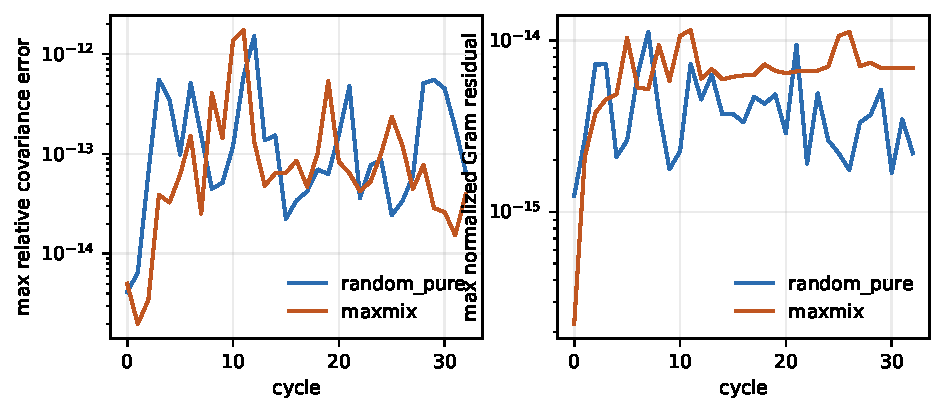
\includegraphics[width=\linewidth]{../figures/correctness_errors.pdf}
\caption{Cycle-resolved covariance and Gram errors.}
\end{figure}

\section{Uniform-insulator convergence}
The finite-size target projector gives $C_{\rm target}=0.999465$. Cycle-resolved disk-partition real-space Chern estimators are retained independently for all four initialization/backend lanes. Half-system entropy is retained for every lane, while global entropy density supplies the purification diagnostic for the maximally mixed initialization.\\
maxmix.covariance: $C_0=0.0000$, $C_{32}=0.9999$, $S_{
m global}(32)/N=7.373e-16$.\\
maxmix.frame: $C_0=0.0000$, $C_{32}=0.9999$, $S_{
m global}(32)/N=0.000e+00$.\\
random\_pure.covariance: $C_0=0.0715$, $C_{32}=0.9996$, $S_{
m global}(32)/N=1.700e-15$.\\
random\_pure.frame: $C_0=0.0715$, $C_{32}=0.9996$, $S_{
m global}(32)/N=1.009e-16$.\\

\begin{figure}[t]
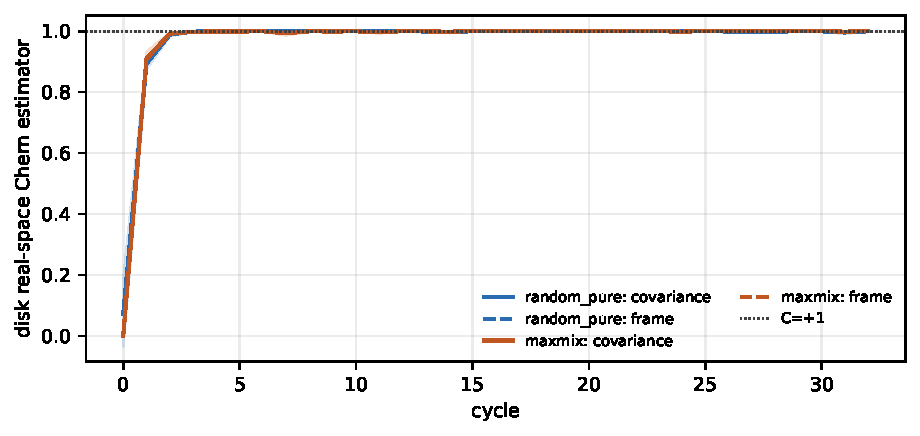
\includegraphics[width=\linewidth]{../figures/chern_convergence_four_lanes.pdf}
\caption{Real-space Chern convergence for the covariance and frame replays of both initial-state families.}
\end{figure}

\section{Performance}
For maxmix, the update-only covariance/frame ratio was 1.029 with paired-bootstrap 95\% interval [1.014,1.043] (comparable); the end-to-end ratio was 1.026 [1.012,1.041] (comparable). For random\_pure, the update-only covariance/frame ratio was 6.285 with paired-bootstrap 95\% interval [5.972,6.648] (faster); the end-to-end ratio was 6.258 [5.953,6.612] (faster). Ratios greater than one favor the frame backend. Classification uses a predeclared $\pm5\%$ practical-equivalence band and the paired-bootstrap interval, with each record as the independent unit.

\section{Limitations}
This study covers a CPU-only $16\times16$, $n_{\rm shell}=1$ uniform controller and 32 cycles. The disk Chern estimator is a finite-size convergence diagnostic; the calibrated target is therefore used instead of assuming an exactly quantized finite-lattice value. Purification frames retain doubled-space costs and may show no speed improvement. Observer Chern contractions, eigendecompositions/SVDs, and diagnostic reconstructions are reported separately from dynamics.

\end{document}
